\documentclass[]{article}
\usepackage{lmodern}
\usepackage{amssymb,amsmath}
\usepackage{ifxetex,ifluatex}
\usepackage{fixltx2e} % provides \textsubscript
\ifnum 0\ifxetex 1\fi\ifluatex 1\fi=0 % if pdftex
  \usepackage[T1]{fontenc}
  \usepackage[utf8]{inputenc}
\else % if luatex or xelatex
  \ifxetex
    \usepackage{mathspec}
  \else
    \usepackage{fontspec}
  \fi
  \defaultfontfeatures{Ligatures=TeX,Scale=MatchLowercase}
\fi
% use upquote if available, for straight quotes in verbatim environments
\IfFileExists{upquote.sty}{\usepackage{upquote}}{}
% use microtype if available
\IfFileExists{microtype.sty}{%
\usepackage{microtype}
\UseMicrotypeSet[protrusion]{basicmath} % disable protrusion for tt fonts
}{}
\usepackage[margin=1in]{geometry}
\usepackage{hyperref}
\hypersetup{unicode=true,
            pdftitle={SSMIF Factor Model User Guide},
            pdfauthor={Anand Patel},
            pdfborder={0 0 0},
            breaklinks=true}
\urlstyle{same}  % don't use monospace font for urls
\usepackage{longtable,booktabs}
\usepackage{graphicx,grffile}
\makeatletter
\def\maxwidth{\ifdim\Gin@nat@width>\linewidth\linewidth\else\Gin@nat@width\fi}
\def\maxheight{\ifdim\Gin@nat@height>\textheight\textheight\else\Gin@nat@height\fi}
\makeatother
% Scale images if necessary, so that they will not overflow the page
% margins by default, and it is still possible to overwrite the defaults
% using explicit options in \includegraphics[width, height, ...]{}
\setkeys{Gin}{width=\maxwidth,height=\maxheight,keepaspectratio}
\IfFileExists{parskip.sty}{%
\usepackage{parskip}
}{% else
\setlength{\parindent}{0pt}
\setlength{\parskip}{6pt plus 2pt minus 1pt}
}
\setlength{\emergencystretch}{3em}  % prevent overfull lines
\providecommand{\tightlist}{%
  \setlength{\itemsep}{2pt}\setlength{\parskip}{0pt}}
\setcounter{secnumdepth}{5}
\linespread{1.3}
% Redefines (sub)paragraphs to behave more like sections
\ifx\paragraph\undefined\else
\let\oldparagraph\paragraph
\renewcommand{\paragraph}[1]{\oldparagraph{#1}\mbox{}}
\fi
\ifx\subparagraph\undefined\else
\let\oldsubparagraph\subparagraph
\renewcommand{\subparagraph}[1]{\oldsubparagraph{#1}\mbox{}}
\fi

%%% Use protect on footnotes to avoid problems with footnotes in titles
\let\rmarkdownfootnote\footnote%
\def\footnote{\protect\rmarkdownfootnote}

%%% Change title format to be more compact
\usepackage{titling}

% Create subtitle command for use in maketitle
\providecommand{\subtitle}[1]{
  \posttitle{
    \begin{center}\large#1\end{center}
    }
}

\setlength{\droptitle}{-2em}

  \title{SSMIF Factor Model - User Guide}
    \pretitle{\vspace{\droptitle}\centering\huge}
  \posttitle{\par}
    \author{Written by: Anand Patel, Head of Factor Model (Spring 2020)}
    \preauthor{\centering\large\emph}
  \postauthor{\par}
    \date{}
    \predate{}\postdate{}
  
\usepackage{graphicx}
\usepackage{float}

\begin{document}
\maketitle

\hypertarget{introduction}{%
\section{Introduction}\label{introduction}}

The ultimate goal of the SSMIF's factor model is to inform Senior
Management on investment decisions by providing optimal allocations
across the sectors of the S\&P 500 (excluding real estate). In order to
do so, the model uses as much valuation and sentiment data as is
available since 1990 in addition to macroeconomic data to model the
movement and performance of each sector. Movemenent is predicted using
three different models, all the models' predictions are blended together
and used in a genetic optimization technique that scores different
combinations of sector weights using an objective function that takes
into account returns, volatility, VaR, and CVaR all relative to the
fund's benchmark, the S\&P 500. Once the optimization is completed, we
have our optimal sector allocations and we can run them through a
backtest which calculates various statistics and generates graphics that
provide information about performance of the models as well as the
constructed portfolio.

The code in this repository \textbf{should} be sufficiently commented so
that future members of the QIS team, specifically those that will work
on the factor model, can understand the code and what everything is
meant to do. This document is meant to be supplemental in case comments
aren't clear enough, or as a general guide for anyone within the fund
that wants a more in-depth understanding of the factor model.


\hypertarget{detailed-methodology}{%
\section{Detailed Methodology}\label{detailed-methodology}}

\hypertarget{data-collection}{%
\subsection{Data Collection}\label{data-collection}}

\textbf{\emph{Relevant files:}} \texttt{DataLoad.R}

\hypertarget{retrieving-data-from-bloomberg}{%
\subsubsection{Retrieving Data From
Bloomberg}\label{retrieving-data-from-bloomberg}}

Ideally, the factor model should be run on a Bloomberg Terminal so that
the most up-to-date data is being used, but in practice, once a week
should be fine when experimenting with the model just to make sure it
can still handle new data as expected (Note: make sure you're logged
into the Bloomberg software, and that the BBComm service is running so
that it can communicate with the API we are using). If on a Terminal,
all the data is retrieved by factor category (valuation, sentiment,
macroeconomic) on a per-sector level and cleaned based on what type of
factor it is:

\begin{itemize}
\item
  \textbf{Valuation Data:} For valuation data, just the weekends and
  market holidays/closures are removed so it doesn't have to be done
  every time the file is loaded again.
\item
  \textbf{Sentiment Data:} This data is retrieved using the S\&P 500
  sector ETFs (eg. ``XLK US Equity'') as proxies since the indices we
  use for the valuation data aren't exchange-traded. With the ETFs, we
  can access the sentiment-related data we're looking for, including the
  percentage of shares which are owned by institutions, the total volume
  traded and the put-call open interest ratio of the options on those
  ETFs. For insititutional ownership, the data is only reported on
  Sundays beginning in March 2010 (except Communication Services, since
  its constituents were changed around in the summer of 2018 according
  to changes in the GICS), so we copy each Sunday's level and extend it
  to the rest of that week.
\item
  \textbf{Macroeconomic Data:} Similar to the sentiment data, a lot of
  the macro data we collect is measured and reported at a lower
  frequency than the rest of the data, so for each of those fields, the
  value is extended for the entire month/quarter.
\end{itemize}

Once the data for each factor category is cleaned and processed, it is
all written to CSV files in corresponding folders under the
\texttt{data/} directory. Also collected is the most recent daily data
for the SPX Index and each sector's index (eg. ``S5INFT Index'' for the
IT sector), which are saved in \texttt{data/SPX.csv} and
\texttt{data/sectors.csv} respectively. The motive behind saving all the
data to files (and not just use the data directly) is that it allows you
to work with the model on your own computer and not just when you're in
the Hanlon labs.

\hypertarget{loading-locally-saved-data}{%
\subsubsection{Loading Locally-Saved
Data}\label{loading-locally-saved-data}}

Regardless of whether or not you're on a Bloomberg Terminal, the data is
loaded from the saved files for preparation to use in the models. Most
of the heavy lifting here has to do with making sure the data is
formatted so it can be merged properly, as well as calculating some of
the derived factors, such as PEG (or what is supposed to be PEG, the
factor model when I first started working on it actually calculates this
as \(\frac{Price}{FCF\; Yield}\). We tried fixing this so it finds
\(PEG=\frac{P/E\; ratio}{EPS\; growth\; rate}\), but the model results
became far less accurate, so it was kept as
\(\frac{Price}{FCF\; Yield}\). Finally, once the valuation, sentiment,
and macroeconomic data are all merged for each sector, it is split up in
a roughly 70/30 split into training and testing data, and then we are
ready to move onto modelling.

\hypertarget{modelling}{%
\subsection{Modelling}\label{modelling}}

\textbf{\emph{Relevant files:}} \texttt{linearAnalysis.R},
\texttt{arimaAnalysis.R}, \texttt{randomForestAnalysis.R}

The actual modelling that we do is split across three different methods:
a linear regression, an ARIMA time series model, as well as a random
forest regression. The methodology for each of these is pretty standard:
each model is fitted using the training data, predictions are generated
across the domain of the testing period, then we measure error between
the model predictions and actual values of each sector index. The error
measure was recently changed to the log of the accuracy ratio
\(log(\frac{prediction}{actual})\). Previously, we had used mean
absolute percentage error, but after some research, we found MAPE was a
biased metric in that
\href{https://papers.ssrn.com/sol3/papers.cfm?abstract_id=2635088}{it
would favor models with predictions that are systematically too low},
leading to using the symmetric log-based measure.

\hypertarget{model-construction}{%
\subsubsection{Model Construction}\label{model-construction}}

The model we construct and regressors used are consistent across every
sector, and used in both the linear regression and later on for the
random forest regression. Currently, the linear and random forest models
are constructed as follows:

\[
ln(Price) = \beta^T
\begin{pmatrix}
PE \\
PB \\
PS \\
FCF\;Yield \\
PEG \\
Debt/Asset\; \% \\
Earnings\; Yield \\
Volume \\
GDP\; Growth \\
2y\; Treasury\; Yield \\
10y\; Treasury\; Yield \\
Unemployment\; Rate \\
LFPR \\
Consumer\; Sentiment \\
Inflation
\end{pmatrix}
\]

where \(\beta\) is the vector of coefficients that are generated when
the model is fitted for each sector. The ARIMA models are similar, with
additional terms
\(\phi_0+\sum_{i=1}^{p}{\phi_i log(Price)_{t-i}+\epsilon_t}\) and
\(\mu+\epsilon_t+\sum_{i=1}^{q}{\theta_t\epsilon_{t-i}}\) to capture the
AR and MA movement, respectively.

Once the models are all fitted using the training data, we generate the
predictions for each model so that we can measure the error of each, and
ultimately optimize how those predictions are blended together. The loss
function that we use as a measure of error is as follows:

\[Error = \sum_{i=1}^{N} ln(\frac{Predicted\; Price}{Actual\; Price})^2\]

For reference, the calculated errors per sector per model (as of
February 28, 2020) is as follows:

\begin{longtable}[]{@{}cccc@{}}
\toprule
& LIN & ARIMA & RF\tabularnewline
\midrule
\endhead
\textbf{IT} & 14.5854 & 0.2284 & 35.2586\tabularnewline
\textbf{FIN} & 16.1205 & 2.8901 & 14.0032\tabularnewline
\textbf{ENG} & 2.1826 & 5.3581 & 17.1124\tabularnewline
\textbf{HLTH} & 0.4087 & 0.0531 & 37.2373\tabularnewline
\textbf{CONS} & 0.0821 & 3.0412 & 35.6733\tabularnewline
\textbf{COND} & 0.3226 & 0.5113 & 42.3518\tabularnewline
\textbf{INDU} & 4.0867 & 0.0946 & 30.8783\tabularnewline
\textbf{UTIL} & 8.9123 & 0.2795 & 9.349\tabularnewline
\textbf{TELS} & 8.5881 & 3.6411 & 4.0634\tabularnewline
\textbf{MATR} & 1.2418 & 1.8983 & 12.8529\tabularnewline
\bottomrule
\end{longtable}

\hypertarget{blending-model-predictions}{%
\subsubsection{Blending Model
Predictions}\label{blending-model-predictions}}

Since we use three modelling methods, we have to combine the predictions
made by each into a master set of predictions over the testing period,
which will ultimately be used in the optimization method. Since we
measure error for each model, we want to give more weight to the model
whose predictions have lower errors than those with higher errors.

To do so, we implement an inverse weighted average method that does
exactly this by calculating the inverse percentage of each model's error
across all the models for that sector, then dividing each of those
``factors'' by the sum of all factors for that sector. Using an example
(COND) makes this concept easier to understand:

\[
Factor=\begin{pmatrix}
\frac{0.3226+0.5113+42.3518}{0.3226} \\
\\
\frac{0.3226+0.5113+42.3518}{0.5113} \\
\\
\frac{0.3226+0.5113+42.3518}{42.3518}
\end{pmatrix} =
\begin{pmatrix}
133.86764  \\
84.46255 \\
1.01969
\end{pmatrix}
\]

\[
Weight=\begin{pmatrix}
\frac{133.86764}{133.86764+84.46255+1.01969} \\
\\
\frac{84.46255}{133.86764+84.46255+1.01969} \\
\\
\frac{1.01969}{133.86764+84.46255+1.01969}
\end{pmatrix}=
\begin{pmatrix}
0.6103  \\
0.3851 \\
0.0046
\end{pmatrix}
\]

\[
Overall\;Error=\begin{pmatrix}0.3226 & 0.5113 & 42.3518\end{pmatrix}
\begin{pmatrix}0.6103 \\ 0.3851 \\ 0.0046\end{pmatrix}
= 0.0648
\]

As expected, the random forest model, which has an astronomically high
error compared to the linear regression and ARIMA analysis, gets almost
zero weight while the lowest error from the linear regression gets over
60\% weight towards the overall error and the predictions.

Using the February 28th data again, these are the factors, model
weights, and overall errors for each sector:

\begin{longtable}[]{@{}ccccllll@{}}
\toprule
\begin{minipage}[b]{0.05\columnwidth}\centering
\strut
\end{minipage} & \begin{minipage}[b]{0.10\columnwidth}\centering
LIN Factor\strut
\end{minipage} & \begin{minipage}[b]{0.12\columnwidth}\centering
ARIMA Factor\strut
\end{minipage} & \begin{minipage}[b]{0.09\columnwidth}\centering
RF Factor\strut
\end{minipage} & \begin{minipage}[b]{0.10\columnwidth}\raggedright
LIN Weight\strut
\end{minipage} & \begin{minipage}[b]{0.12\columnwidth}\raggedright
ARIMA Weight\strut
\end{minipage} & \begin{minipage}[b]{0.09\columnwidth}\raggedright
RF Weight\strut
\end{minipage} & \begin{minipage}[b]{0.12\columnwidth}\raggedright
Overall Error\strut
\end{minipage}\tabularnewline
\midrule
\endhead
\begin{minipage}[t]{0.05\columnwidth}\centering
\textbf{IT}\strut
\end{minipage} & \begin{minipage}[t]{0.10\columnwidth}\centering
3.517\strut
\end{minipage} & \begin{minipage}[t]{0.12\columnwidth}\centering
224.579\strut
\end{minipage} & \begin{minipage}[t]{0.09\columnwidth}\centering
1.406\strut
\end{minipage} & \begin{minipage}[t]{0.10\columnwidth}\raggedright
1.53\%\strut
\end{minipage} & \begin{minipage}[t]{0.12\columnwidth}\raggedright
97.85\%\strut
\end{minipage} & \begin{minipage}[t]{0.09\columnwidth}\raggedright
0.61\%\strut
\end{minipage} & \begin{minipage}[t]{0.12\columnwidth}\raggedright
\textbf{0.1668}\strut
\end{minipage}\tabularnewline
\begin{minipage}[t]{0.05\columnwidth}\centering
\textbf{FIN}\strut
\end{minipage} & \begin{minipage}[t]{0.10\columnwidth}\centering
2.113\strut
\end{minipage} & \begin{minipage}[t]{0.12\columnwidth}\centering
11.788\strut
\end{minipage} & \begin{minipage}[t]{0.09\columnwidth}\centering
2.263\strut
\end{minipage} & \begin{minipage}[t]{0.10\columnwidth}\raggedright
13.07\%\strut
\end{minipage} & \begin{minipage}[t]{0.12\columnwidth}\raggedright
72.93\%\strut
\end{minipage} & \begin{minipage}[t]{0.09\columnwidth}\raggedright
14.00\%\strut
\end{minipage} & \begin{minipage}[t]{0.12\columnwidth}\raggedright
\textbf{4.2259}\strut
\end{minipage}\tabularnewline
\begin{minipage}[t]{0.05\columnwidth}\centering
\textbf{ENG}\strut
\end{minipage} & \begin{minipage}[t]{0.10\columnwidth}\centering
10.692\strut
\end{minipage} & \begin{minipage}[t]{0.12\columnwidth}\centering
4.355\strut
\end{minipage} & \begin{minipage}[t]{0.09\columnwidth}\centering
1.477\strut
\end{minipage} & \begin{minipage}[t]{0.10\columnwidth}\raggedright
64.70\%\strut
\end{minipage} & \begin{minipage}[t]{0.12\columnwidth}\raggedright
26.36\%\strut
\end{minipage} & \begin{minipage}[t]{0.09\columnwidth}\raggedright
8.94\%\strut
\end{minipage} & \begin{minipage}[t]{0.12\columnwidth}\raggedright
\textbf{1.2395}\strut
\end{minipage}\tabularnewline
\begin{minipage}[t]{0.05\columnwidth}\centering
\textbf{HLTH}\strut
\end{minipage} & \begin{minipage}[t]{0.10\columnwidth}\centering
89.032\strut
\end{minipage} & \begin{minipage}[t]{0.12\columnwidth}\centering
685.14\strut
\end{minipage} & \begin{minipage}[t]{0.09\columnwidth}\centering
1.013\strut
\end{minipage} & \begin{minipage}[t]{0.10\columnwidth}\raggedright
11.49\%\strut
\end{minipage} & \begin{minipage}[t]{0.12\columnwidth}\raggedright
88.38\%\strut
\end{minipage} & \begin{minipage}[t]{0.09\columnwidth}\raggedright
0.13\%\strut
\end{minipage} & \begin{minipage}[t]{0.12\columnwidth}\raggedright
\textbf{0.0487}\strut
\end{minipage}\tabularnewline
\begin{minipage}[t]{0.05\columnwidth}\centering
\textbf{CONS}\strut
\end{minipage} & \begin{minipage}[t]{0.10\columnwidth}\centering
476.546\strut
\end{minipage} & \begin{minipage}[t]{0.12\columnwidth}\centering
12.869\strut
\end{minipage} & \begin{minipage}[t]{0.09\columnwidth}\centering
1.087\strut
\end{minipage} & \begin{minipage}[t]{0.10\columnwidth}\raggedright
97.15\%\strut
\end{minipage} & \begin{minipage}[t]{0.12\columnwidth}\raggedright
2.62\%\strut
\end{minipage} & \begin{minipage}[t]{0.09\columnwidth}\raggedright
0.22\%\strut
\end{minipage} & \begin{minipage}[t]{0.12\columnwidth}\raggedright
\textbf{0.0762}\strut
\end{minipage}\tabularnewline
\begin{minipage}[t]{0.05\columnwidth}\centering
\textbf{COND}\strut
\end{minipage} & \begin{minipage}[t]{0.10\columnwidth}\centering
137.563\strut
\end{minipage} & \begin{minipage}[t]{0.12\columnwidth}\centering
88.789\strut
\end{minipage} & \begin{minipage}[t]{0.09\columnwidth}\centering
1.019\strut
\end{minipage} & \begin{minipage}[t]{0.10\columnwidth}\raggedright
61.04\%\strut
\end{minipage} & \begin{minipage}[t]{0.12\columnwidth}\raggedright
38.51\%\strut
\end{minipage} & \begin{minipage}[t]{0.09\columnwidth}\raggedright
0.45\%\strut
\end{minipage} & \begin{minipage}[t]{0.12\columnwidth}\raggedright
\textbf{0.0648}\strut
\end{minipage}\tabularnewline
\begin{minipage}[t]{0.05\columnwidth}\centering
\textbf{INDU}\strut
\end{minipage} & \begin{minipage}[t]{0.10\columnwidth}\centering
9.031\strut
\end{minipage} & \begin{minipage}[t]{0.12\columnwidth}\centering
390.024\strut
\end{minipage} & \begin{minipage}[t]{0.09\columnwidth}\centering
1.128\strut
\end{minipage} & \begin{minipage}[t]{0.10\columnwidth}\raggedright
2.26\%\strut
\end{minipage} & \begin{minipage}[t]{0.12\columnwidth}\raggedright
97.46\%\strut
\end{minipage} & \begin{minipage}[t]{0.09\columnwidth}\raggedright
0.28\%\strut
\end{minipage} & \begin{minipage}[t]{0.12\columnwidth}\raggedright
\textbf{0.0959}\strut
\end{minipage}\tabularnewline
\begin{minipage}[t]{0.05\columnwidth}\centering
\textbf{UTIL}\strut
\end{minipage} & \begin{minipage}[t]{0.10\columnwidth}\centering
2.071\strut
\end{minipage} & \begin{minipage}[t]{0.12\columnwidth}\centering
66.017\strut
\end{minipage} & \begin{minipage}[t]{0.09\columnwidth}\centering
1.993\strut
\end{minipage} & \begin{minipage}[t]{0.10\columnwidth}\raggedright
2.95\%\strut
\end{minipage} & \begin{minipage}[t]{0.12\columnwidth}\raggedright
94.20\%\strut
\end{minipage} & \begin{minipage}[t]{0.09\columnwidth}\raggedright
2.84\%\strut
\end{minipage} & \begin{minipage}[t]{0.12\columnwidth}\raggedright
\textbf{0.4230}\strut
\end{minipage}\tabularnewline
\begin{minipage}[t]{0.05\columnwidth}\centering
\textbf{TELS}\strut
\end{minipage} & \begin{minipage}[t]{0.10\columnwidth}\centering
1.926\strut
\end{minipage} & \begin{minipage}[t]{0.12\columnwidth}\centering
4.544\strut
\end{minipage} & \begin{minipage}[t]{0.09\columnwidth}\centering
3.836\strut
\end{minipage} & \begin{minipage}[t]{0.10\columnwidth}\raggedright
18.69\%\strut
\end{minipage} & \begin{minipage}[t]{0.12\columnwidth}\raggedright
44.08\%\strut
\end{minipage} & \begin{minipage}[t]{0.09\columnwidth}\raggedright
37.22\%\strut
\end{minipage} & \begin{minipage}[t]{0.12\columnwidth}\raggedright
\textbf{3.7891}\strut
\end{minipage}\tabularnewline
\begin{minipage}[t]{0.05\columnwidth}\centering
\textbf{MATR}\strut
\end{minipage} & \begin{minipage}[t]{0.10\columnwidth}\centering
12.479\strut
\end{minipage} & \begin{minipage}[t]{0.12\columnwidth}\centering
8.164\strut
\end{minipage} & \begin{minipage}[t]{0.09\columnwidth}\centering
1.254\strut
\end{minipage} & \begin{minipage}[t]{0.10\columnwidth}\raggedright
56.99\%\strut
\end{minipage} & \begin{minipage}[t]{0.12\columnwidth}\raggedright
37.28\%\strut
\end{minipage} & \begin{minipage}[t]{0.09\columnwidth}\raggedright
5.73\%\strut
\end{minipage} & \begin{minipage}[t]{0.12\columnwidth}\raggedright
\textbf{0.9558}\strut
\end{minipage}\tabularnewline
\bottomrule
\end{longtable}

\hypertarget{model-accuracy}{%
\subsubsection{Model Accuracy}\label{model-accuracy}}

To help keep track of how these models are performing, and to make it
easier to interpret model performance, we created a graphic that
illustrates the cumulative return of each sector during the testing
period as predicted by the models versus the actual return:

\begin{figure}[H]
\centering
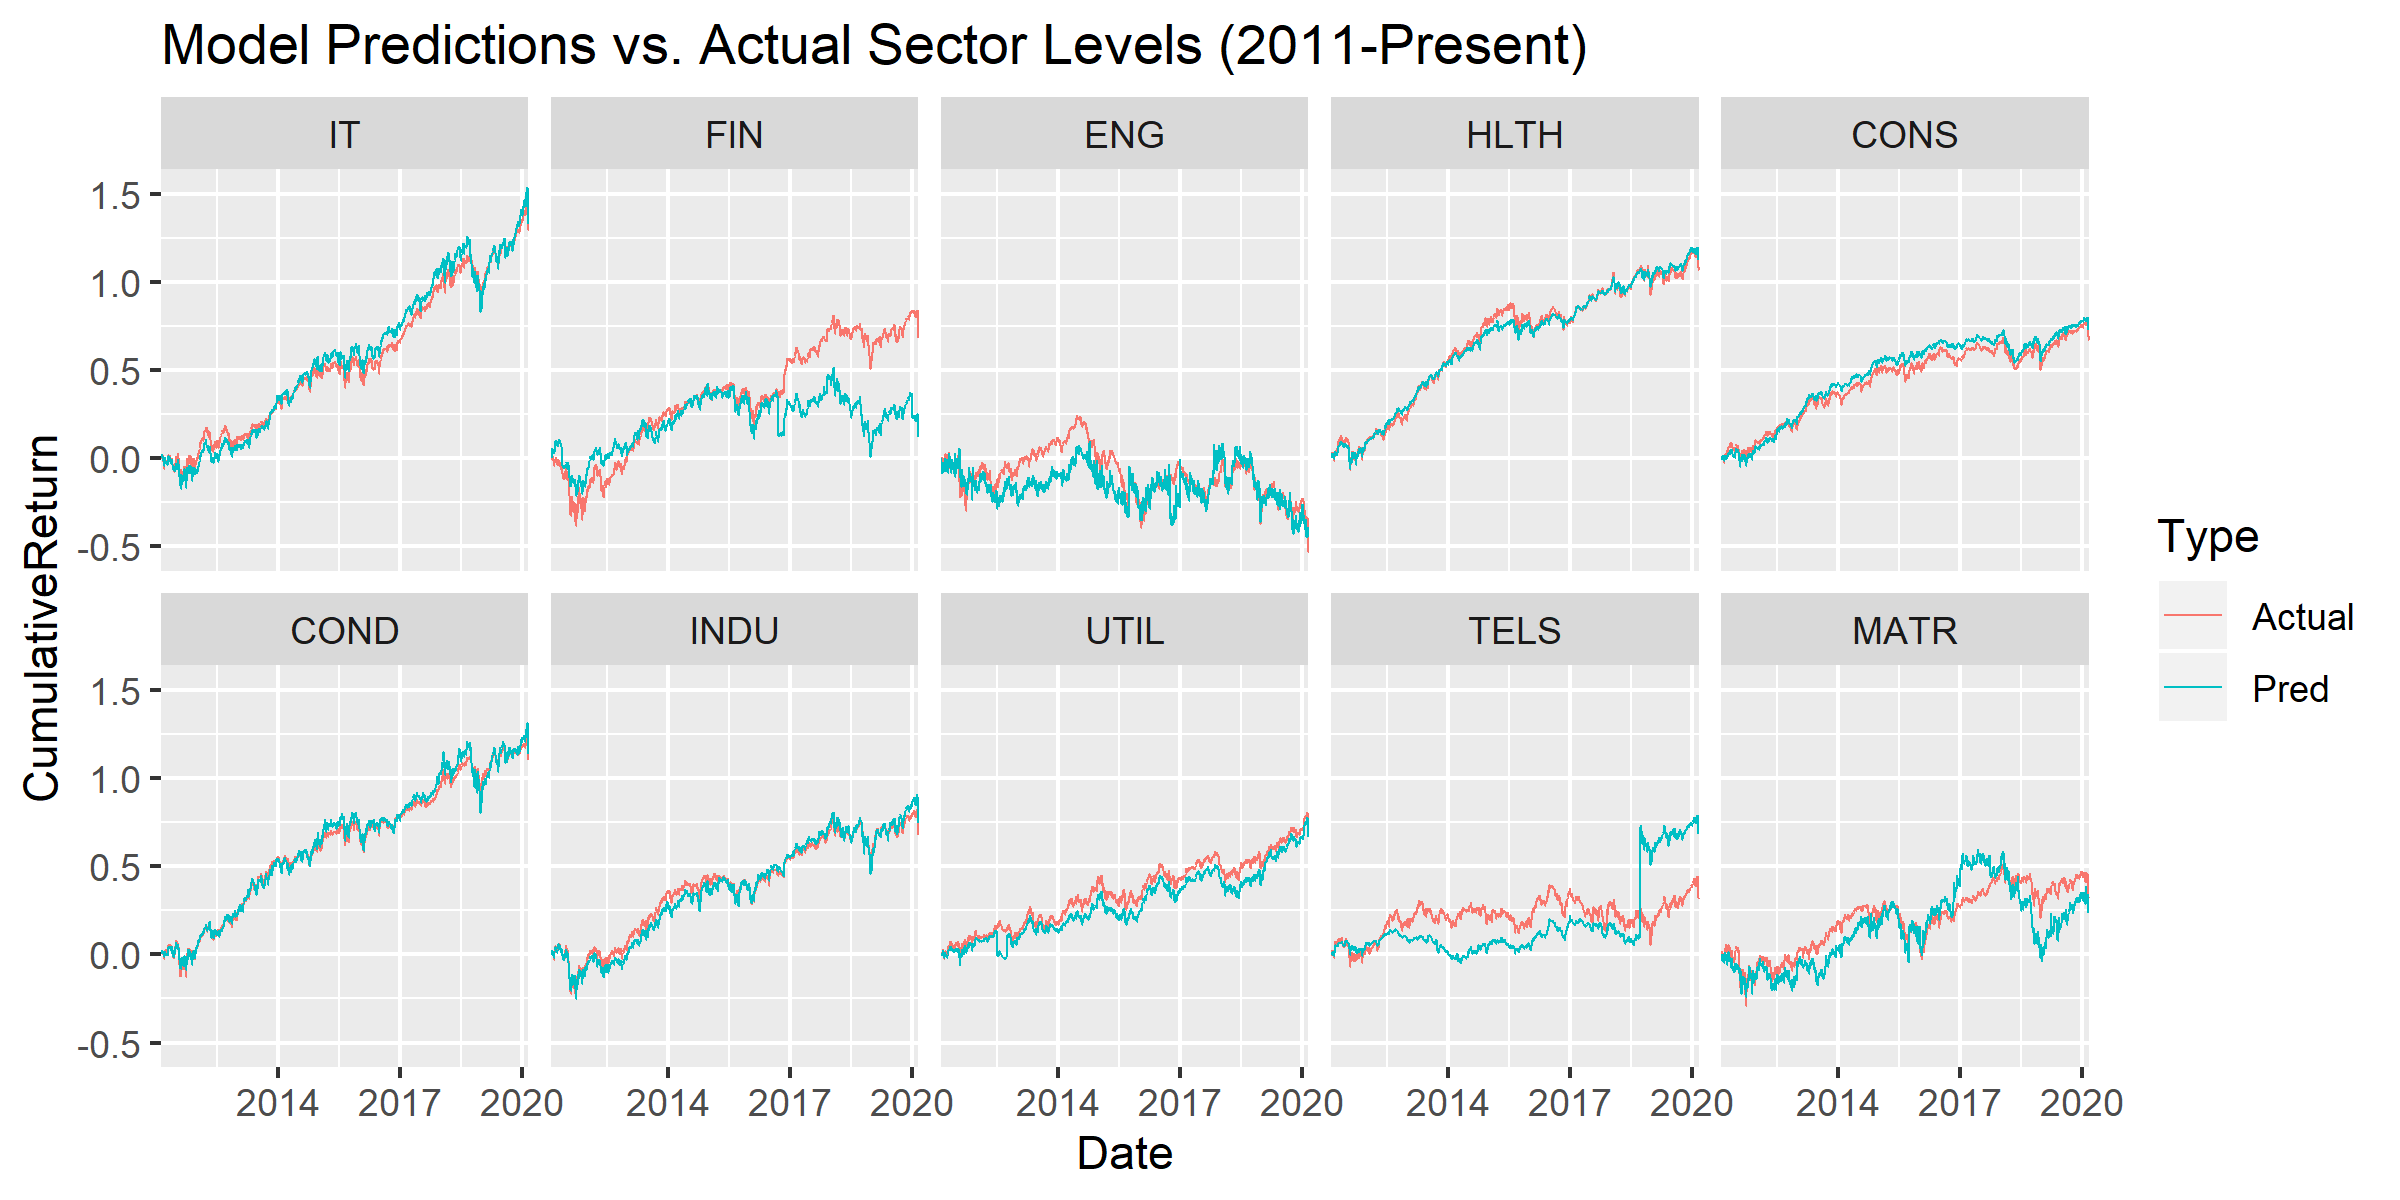
\includegraphics{./results/20200228/modelAssessment.png}
\caption{Illustrative model performance}
\end{figure}

As we can see, the models do a good job of predicted the movement of
each sector, with a few exceptions: 

\begin{itemize}
\item\textbf{Financials}: the financial
sector predictions begin to diverge in late 2016 - likely due to the
presidential election, which caused the market to rally around bank
stocks in anticipation of financial deregulation. Here, the ARIMA
model's predictions were weighted the most, and gave all the sentiment
factors either little to no contribution in the model because of so much
missing data in the training period - meaning that the model couldn't
capture what was a sentiment-driven rally in that sector.
\item\textbf{Communication Services}: officially, this was the
Telecommunications sector until late in the summer of 2018 when
significant changes were made to the sector and it was renamed to its
current title. Specifically, companies like Facebook, Netflix, Google,
and Disney were added to this sector, and brought with them much higher
valuation metrics than were in the sector previously dominated by AT\&T
and Verizon, which explains the very clear jump in predicted return
around that time for the sector. 
\item\textbf{Materials}: the models
predictions were more volatile than the actual returns over that time,
which could mean that the optimization gives less weight to that sector
because it still ends up around the 25\% cumulative return the sector
actually achieved, but with higher risk metrics, which the objective
function will penalize it for.
\end{itemize}

\hypertarget{optimization}{%
\subsection{Optimization}\label{optimization}}

\textbf{\emph{Relevant Files}}: \texttt{geneticBreedv2.R}

To find the optimal weights, we employ a genetic breeding algorithm,
which essentially starts out with a set of random weights and ``breeds''
children with them, and then kills off the lowest performing sets of
weights according to our objective function that we are optimizing:

\[
\max\limits_{\omega}
\begin{pmatrix}
0.85 \\
-0.05 \\
0.05 \\
0.05 \\
\end{pmatrix}^T
\begin{pmatrix}
\rho_P - \rho_m \\
|(1-u)\sigma^2_P-\sigma^2_m| \\
VaR^{95\%}_P-VaR^{95\%}_m \\
CVaR^{95\%}_P-CVaR^{95\%}_m \\
\end{pmatrix}
\]

Ultimately, this is optimizing Sharpe ratio, as we are trying to
maximize excess return, 95\% VaR, and CVaR of the portfolio over the
benchmark S\&P 500 while trying to match the market's volatility with
some undershoot percentage \(u\) - this is so we can aim to achieve the
investment goals outlined in the IPS of beating the market with less
risk.

For reference, the previous optimization method used to find the best
weights was through a Monte Carlo simulation that generated 10,000
weights and chose the portfolio with the highest return with less risk
than the market. However, the results from the simulations were far too
random after every run, even when testing on the same dataset. The
genetic algorithm so far has seemed to solve this problem, and in
\texttt{results/weightsHistory.csv}, we started tracking the weekly
factor model outputs, and controlling for some methodology changes over
time, the weights are much more consistent (Note: please don't open the
weights history file using Excel and then save it - Excel automatically
formats the dates, so if you tried to read the file back into R, you'd
run into errors and would have to discard the changes using GitHub).

\hypertarget{genetic-optimization-algorithm}{%
\subsubsection{Genetic Optimization
Algorithm}\label{genetic-optimization-algorithm}}

\begin{enumerate}
\def\labelenumi{\arabic{enumi}.}
\item
  \textbf{Population Generation:} First, we generate and save 6,000
  random weights that abide by our investment policy of no shorts and no
  more than 25\% of the portfolio in a single sector. We generate that
  many as that is the total population size we'll aim to maintain in
  each of the 10 generations that we breed.
\item
  \textbf{Scoring:} In each generation, the first thing we do is score
  each set of weights by plugging them into our objective function. This
  process alone takes more time than everything else in the factor model
  combined, as it involves taking a set of weights, building the
  portfolio and then calculating the return, risk, VaR and CVaR, the
  last two of which are the most intensive. Although each call to
  \texttt{score()} takes only 0.12-0.15 seconds, doing so 6,000 times in
  each generation adds up.
\item
  \textbf{Killing:} The way these weights are optimized is by
  ``killing'' off the least performing ones, and thus breeding children
  from only the best weights in each generation. The current survival
  rate is 1/3, so we find the score in the 67th percentile of the entire
  population, and any set of weights with a score less than that
  threshold is set to null (i.e.~killed off). We keep track of these
  ``kill scores'' and plot them at the end just to confirm that with
  each generation, the threshold rises, meaning we are getting better
  weights each iteration:
\end{enumerate}

\begin{figure}[H]
\begin{center}
\scalebox{0.575}{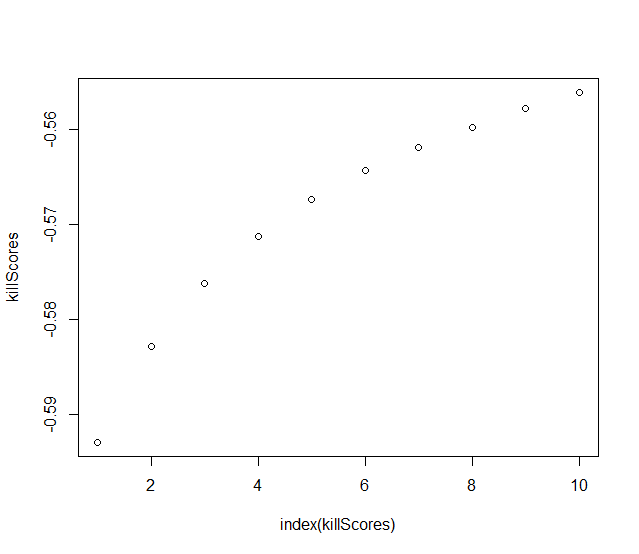
\includegraphics{./results/20200228/killScores.png}}
\caption{Plot of score thresholds for each generation}
\end{center}
\end{figure}

\begin{enumerate}
\def\labelenumi{\arabic{enumi}.}
\setcounter{enumi}{3}
\tightlist
\item
  \textbf{Breeding:} Since only one-third of the population survive, we
  have to regenerate the population until we get back to the target
  6,000, and the following is done in repetition until we do:

  \begin{itemize}
  \tightlist
  \item
    Select two sets of weights at random from the surviving population
  \item
    Breed 3 children from those parent nodes

    \begin{itemize}
    \tightlist
    \item
      Two children come in the following way: for each sector, a random
      number between 0 and 1 is generated, and if it is less than 0.5,
      child A will inherit that sector's weight from parent 1 and child
      B will inherit that sector's weight from parent 2. If the number
      is greater than 0.5, then child A inherits from parent 2 and child
      B inherits from parent 1.
    \item
      The third child C's weights are a simple average of the weights
      from child A and B
    \end{itemize}
  \item
    The children are put through a mutation function, which, with 0.5\%
    probability for each sector, will increase that sector's weight by
    1\% and decrease another random sector by 1\%
  \item
    The rules for the weights are then enforced, so if any of the
    children have negative weights or weights greater than 25\%, the
    child's weights will all be set to zero, which will result in a
    score of \(-\infty\) and definitely be killed off in the next
    generation. The weights of the children are normalized to make sure
    they sum up to 1, so that condition does not have to be checked
    specifically.
  \end{itemize}

  If we are at the tenth and final generation, then we stop the process
  once the bottom 2/3 of the population is killed off, and then choose
  the set of weights corresponding to the maximum score provided by the
  objective function, and then we have our optimal asset allocation
  across the S\&P 500 sectors.
\end{enumerate}

\hypertarget{backtesting}{%
\subsection{Backtesting}\label{backtesting}}

\textbf{\emph{Relevant Files}}: \texttt{fullTest.R}

Backtesting the optimal weights we found involves portfolio statistics
throughout the entire period (1990-present), the testing period (last 9
years), and the current semester. We also generate graphics for most of
the backtest results so we have them for reference as the factor model
continues to evolve and to make it easier for any presentation/report
material should we need to include information on the model.

All graphics below are from February 28, 2020.

\hypertarget{sector-weights}{%
\subsubsection{Sector Weights}\label{sector-weights}}

\begin{figure}[H]
\centering
\scalebox{0.75}{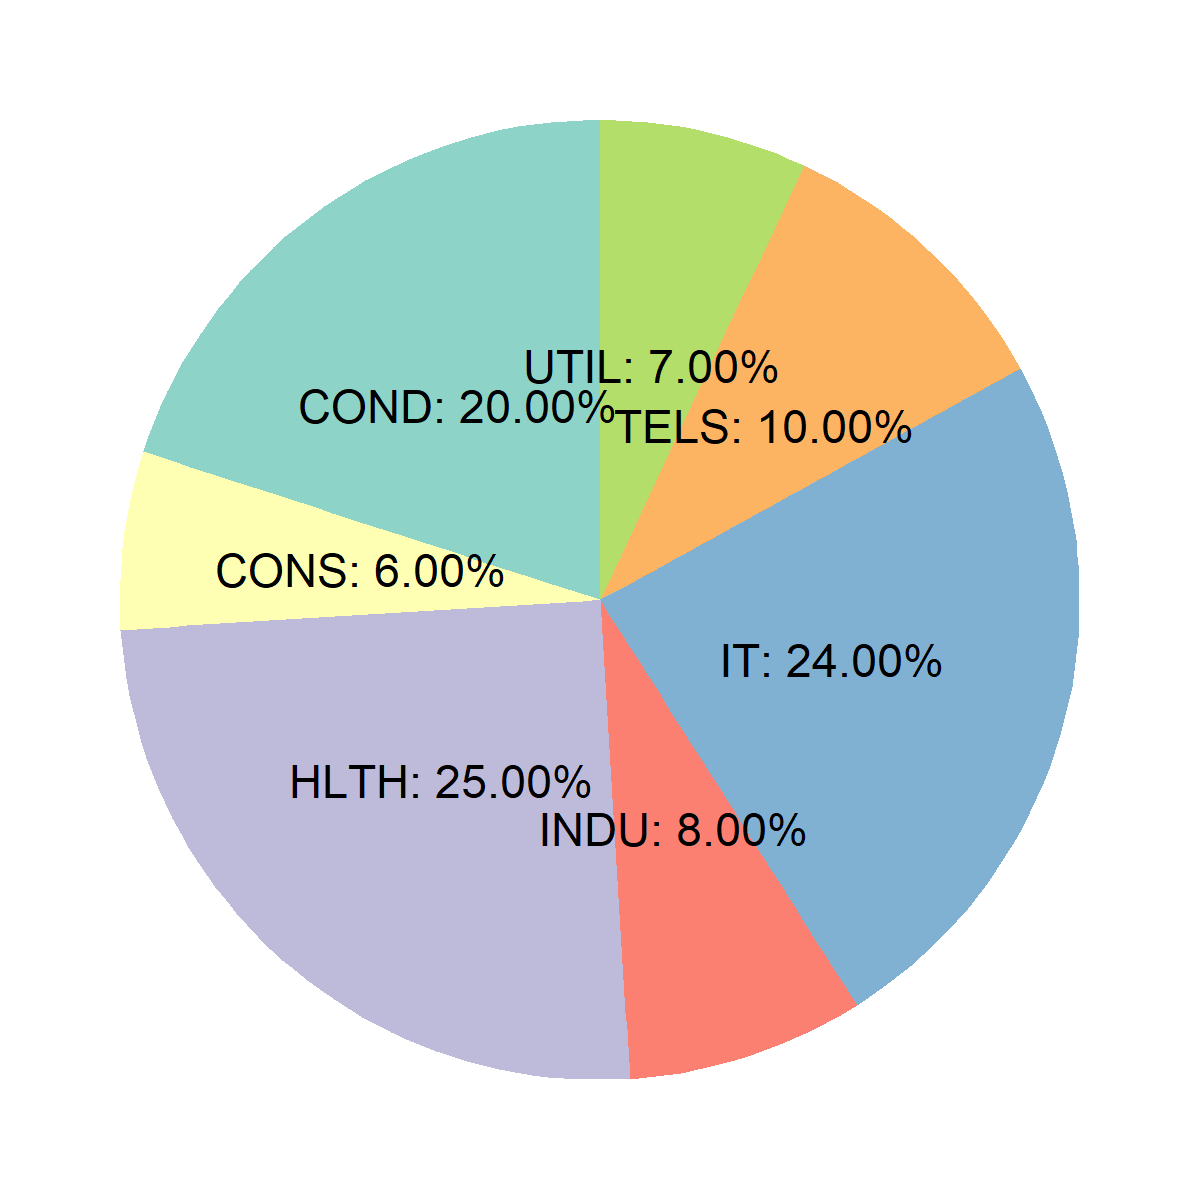
\includegraphics{./results/20200228/weights.png}}
\caption{Pie chart of sector weights}
\end{figure}

As previously mentioned, we also save these weights in
\texttt{results/weightsHistory.csv} to monitor how the weights develop
over time.

\hypertarget{cumulative-return-comparison}{%
\subsubsection{Cumulative Return
Comparison}\label{cumulative-return-comparison}}

\begin{enumerate}
\def\labelenumi{\arabic{enumi}.}
\tightlist
\item
  Overall
\end{enumerate}

\begin{figure}[H]
\centering
\scalebox{0.75}{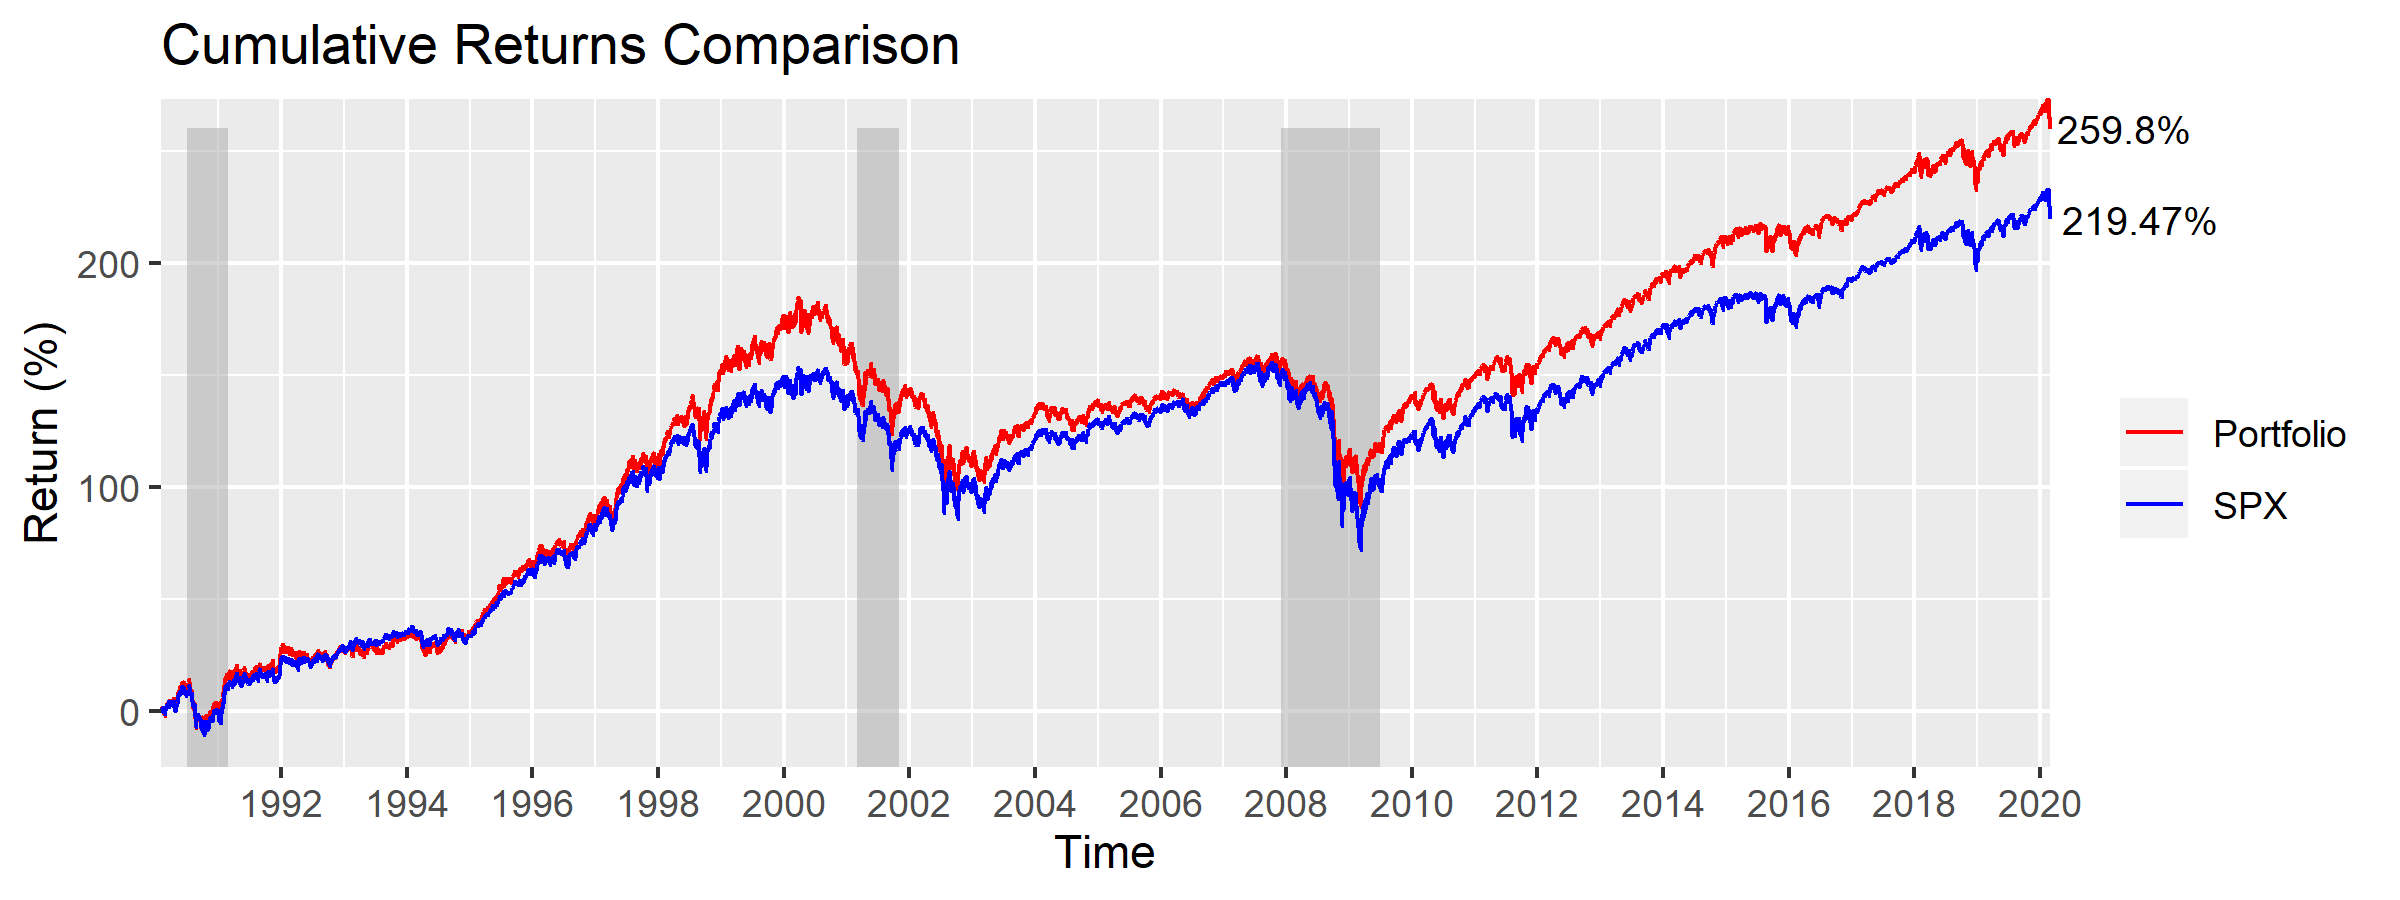
\includegraphics{./results/20200228/cumulativeReturns.png}}
\caption{Overall cumulative return comparison}
\end{figure}

\begin{enumerate}
\def\labelenumi{\arabic{enumi}.}
\setcounter{enumi}{1}
\tightlist
\item
  Testing Period
\end{enumerate}

\begin{figure}[H]
\centering
\scalebox{0.75}{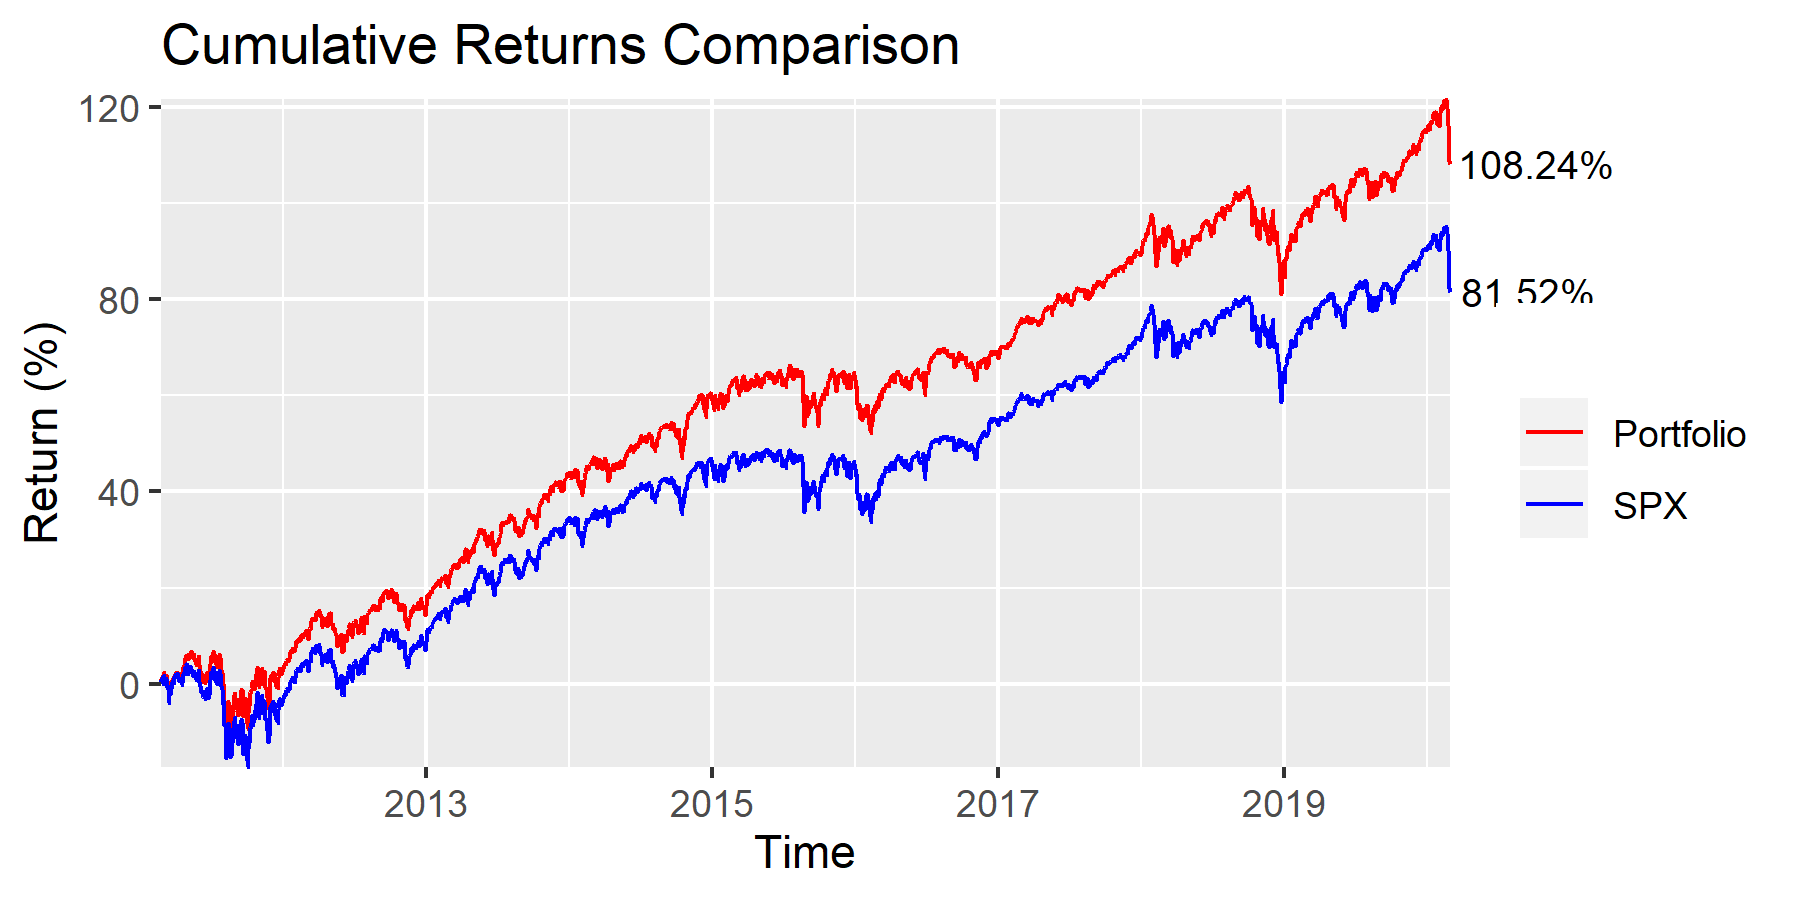
\includegraphics{./results/20200228/cumulativeReturnsTest.png}}
\caption{Testing period cumulative return comparison}
\end{figure}

\begin{enumerate}
\def\labelenumi{\arabic{enumi}.}
\setcounter{enumi}{2}
\tightlist
\item
  Current Semester
\end{enumerate}

\begin{figure}[H]
\centering
\scalebox{0.75}{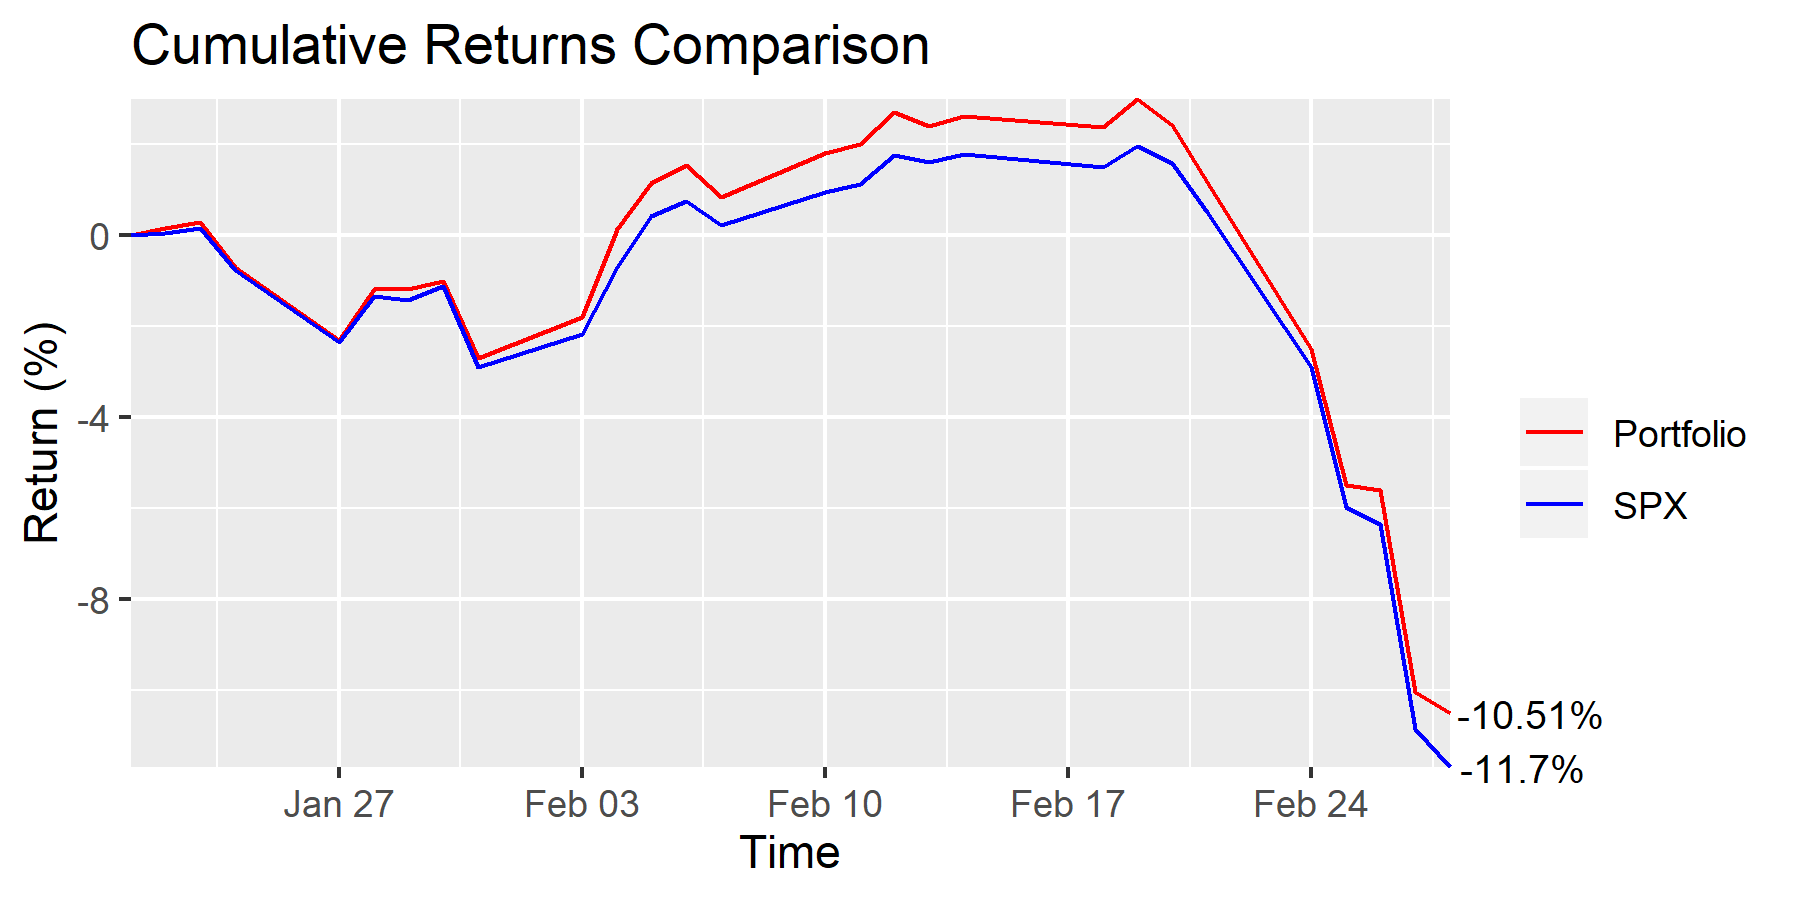
\includegraphics{./results/20200228/cumulativeReturnsSem.png}}
\caption{Semester to date cumulative returns comparison}
\end{figure}

\hypertarget{portfolio-statistics-vs-sp-500}{%
\subsubsection{Portfolio Statistics vs S\&P
500}\label{portfolio-statistics-vs-sp-500}}

Here we save a table of statistics of the portfolio vs the SPX including
cumulative return, total volatility, Sharpe ratio, 95\% VaR and CVaR,
and return comparisons for the three recessions that occurred over the
period we have data for:

\begin{figure}[H]
\centering
\scalebox{0.75}{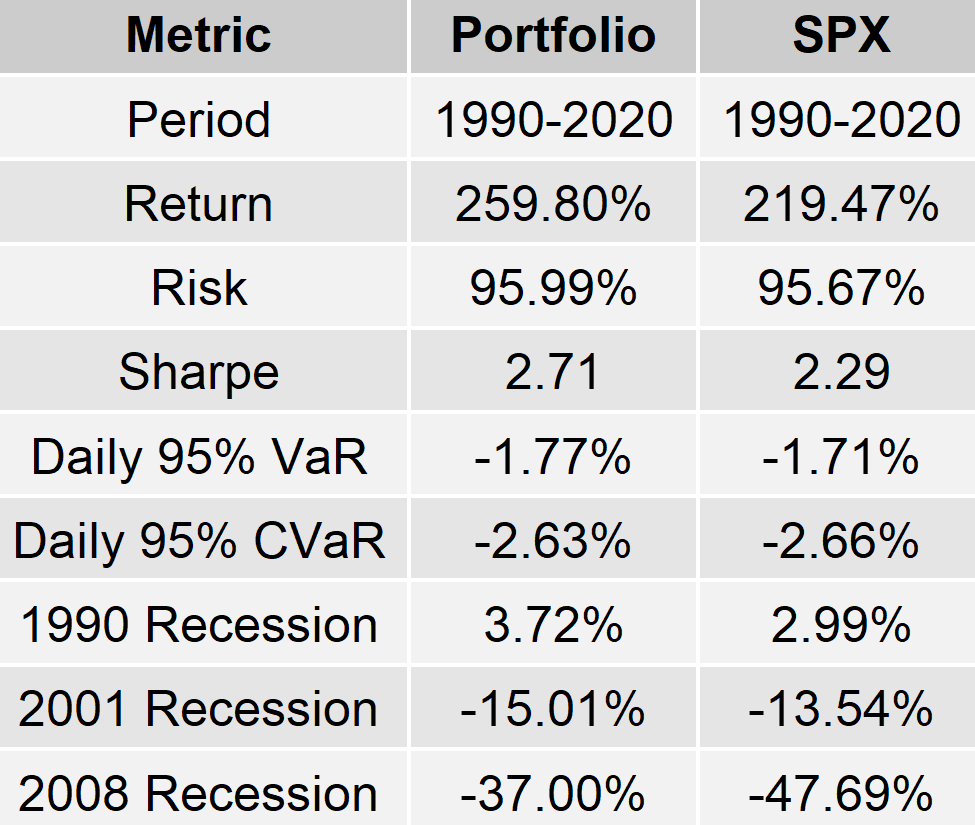
\includegraphics{./results/20200228/stats.png}}
\caption{Portfolio statistics}
\end{figure}

\hypertarget{future-plans}{%
\section{Future Plans}\label{future-plans}}

\begin{itemize}
\tightlist
\item
  Get data on mutual fund inflows and outflows for each sector
  (currently in progress)
\item
  Consolidate some factors like Treasury Yields -- rather than use 2y
  and 10y yields separately, use the 2-10 spread
\item
  Finalize recession probability model and use the output of that as a
  macroeconomic factor in the model
\end{itemize}

\begin{center}
\noindent\rule{8cm}{0.4pt}

\emph{All methodology described above as of Feb 22, 2020}
\end{center}

\end{document}
